%-----------------------------------------------------------%
% Propuesta de plantilla en LaTeX para tesis formato UAG    %
% Autor: Arnulfo Moisés Maciel Hernández                    % 
% Contacto: moy.maciel@gmail.com                            %
% Fecha: Septiembre 2017                                    %
%-----------------------------------------------------------%
% El objetivo de esta plantilla es facilitar la redacción   %
% en LaTeX de tu tesis siguiendo los lineamientos de la UAG.%
% Mi intención es pues que se dedique el tiempo al          %
% contenido de la tesis evitando las largas horas           %
% entendiendo LaTeX.                                        %  
% Siéntete libre de modificar la plantilla de acuerdo a tus %
% necesidades.                                              %
%-----------------------------------------------------------%
% Utiliza el libro libro LaTeX_2014.pdf que se encuentra    %
% dentro de la carpeta "ayuda" para más información.        %
%-----------------------------------------------------------%

%-----------------------------------------------------------%
% Las siguientes configuraciones son con el objetivo de una
% tesis en español siguiendo los lineamientos estipulados
% en: http://crecea.uag.mx/opciones/tesis.htm
% En relación al diseño de la portada los lineamientos 
% estipulados en: http://crecea.uag.mx/opciones/portada.htm

    \documentclass[12pt,twoside]{report}
    \usepackage[utf8]{inputenc}
    \usepackage{pdfpages}
    \usepackage{longtable,multirow,booktabs}
    \usepackage{setspace}
    \usepackage{graphicx}
    \usepackage{cite}
    \usepackage{tabu}
    \usepackage[spanish, es-tabla]{babel}
    \usepackage{amssymb}
    \usepackage{amsmath}
    \usepackage{esvect}
    \usepackage{hyperref}
    \usepackage[a4paper,width=150mm,top=25mm,bottom=25mm,bindingoffset=6mm]{geometry} %Formato márgenes, etc.
    \usepackage[font=footnotesize,labelfont=bf]{caption}
    \usepackage{minted}
    \usepackage{tikz}
    \usepackage{verbatim}
    \graphicspath{{imagenes/}} %Ubicación de imágenes
    \hypersetup{
        %Configuración comandos de referencia cruzada en LATEX:
        colorlinks=true,
        linkcolor=black,
        citecolor=blue,
        filecolor=blue,      
        urlcolor=blue,
        %Opciones de visualización e información PDF:
        pdfauthor={"Tu Nombre va aquí"},
        pdftitle={"El titulo de tu tema de tesis"},
        pdfsubject={"La descripción de tu tema va aquí"},
        pdfcreator={"Tu Nombre va aquí"},
        pdfproducer={"Tu Nombre va aquí"},
        pdfkeywords={"Palabras clave van aquí"}
    }
    
    \begin{document}
    
        %Carátula de tesis

\begin{titlepage}
    \begin{center}
        \rule{\textwidth}{4pt}\vspace*{-\baselineskip}\vspace*{2pt} % Thick horizontal line
        \rule{\textwidth}{1pt}\\[\baselineskip] % Thin horizontal line
        \textbf{\normalsize UNIVERSIDAD AUTÓNOMA DE GUADALAJARA} % Title
        \rule{\textwidth}{0.4pt}\vspace*{-\baselineskip}\vspace{3.2pt} % Thin horizontal line
        \rule{\textwidth}{1.6pt}\\[\baselineskip] % Thick horizontal line
        
        {\tiny CON RECONOCIMIENTO DE VALIDEZ OFICIAL DE ESTUDIOS DE LA SECRETARÍA DE \\ EDUCACIÓN PÚBLICA SEGÚN ACUERDO No.158 DE FECHA 17 DE JULIO DE 1991} % Title
        \rule{\textwidth}{0.4pt}\vspace*{-\baselineskip}\vspace{3.2pt} % Thin horizontal line
        \rule{\textwidth}{1.6pt}\\[\baselineskip] % Thick horizontal line

        \textbf{\small POSTGRADO E INVESTIGACIÓN} % Title
        
        \vspace*{1.2cm}
        
\includegraphics[width=0.3\textwidth]{uag_2.jpg}
        \vspace*{1.2cm}
        
        {\small Aquí es donde escribes el titulo de tu tesis \\ aquí es donde escribes el titulo de tu tesis}
        \rule{\textwidth}{0.6pt}\\[\baselineskip] % Thick horizontal line
        
        \textbf{\small PROYECTO DE INTERVENCIÓN} % Title
        \vspace*{1.2cm} 
        
        {\scriptsize QUE PRESENTA}
        
        \textbf{\scriptsize EDUARDO ALBERTO RODRÍGUEZ GARCÍA }
        \vspace*{1.2cm}
        
        {\scriptsize PARA OBTENER EL GRADO DE}
        
        \textbf{\small MAESTRÍA EN CIENCIAS COMPUTACIONALES} % Title
        \vspace*{1.2cm}
        
        {\scriptsize DIRECTOR Y ASESOR:\\ LINA MARIA AGUILAR LOBO \\ NOMBRE COMPLETO 2}
        
        \vfill
        
        {\scriptsize GUADALAJARA, JALISCO. MARZO 2022 \\ Número de registro en el sistema de investigación}
        \rule{\textwidth}{4pt}\vspace*{-\baselineskip}\vspace*{2pt} % Thick horizontal line
    \end{center}
\end{titlepage}
    
        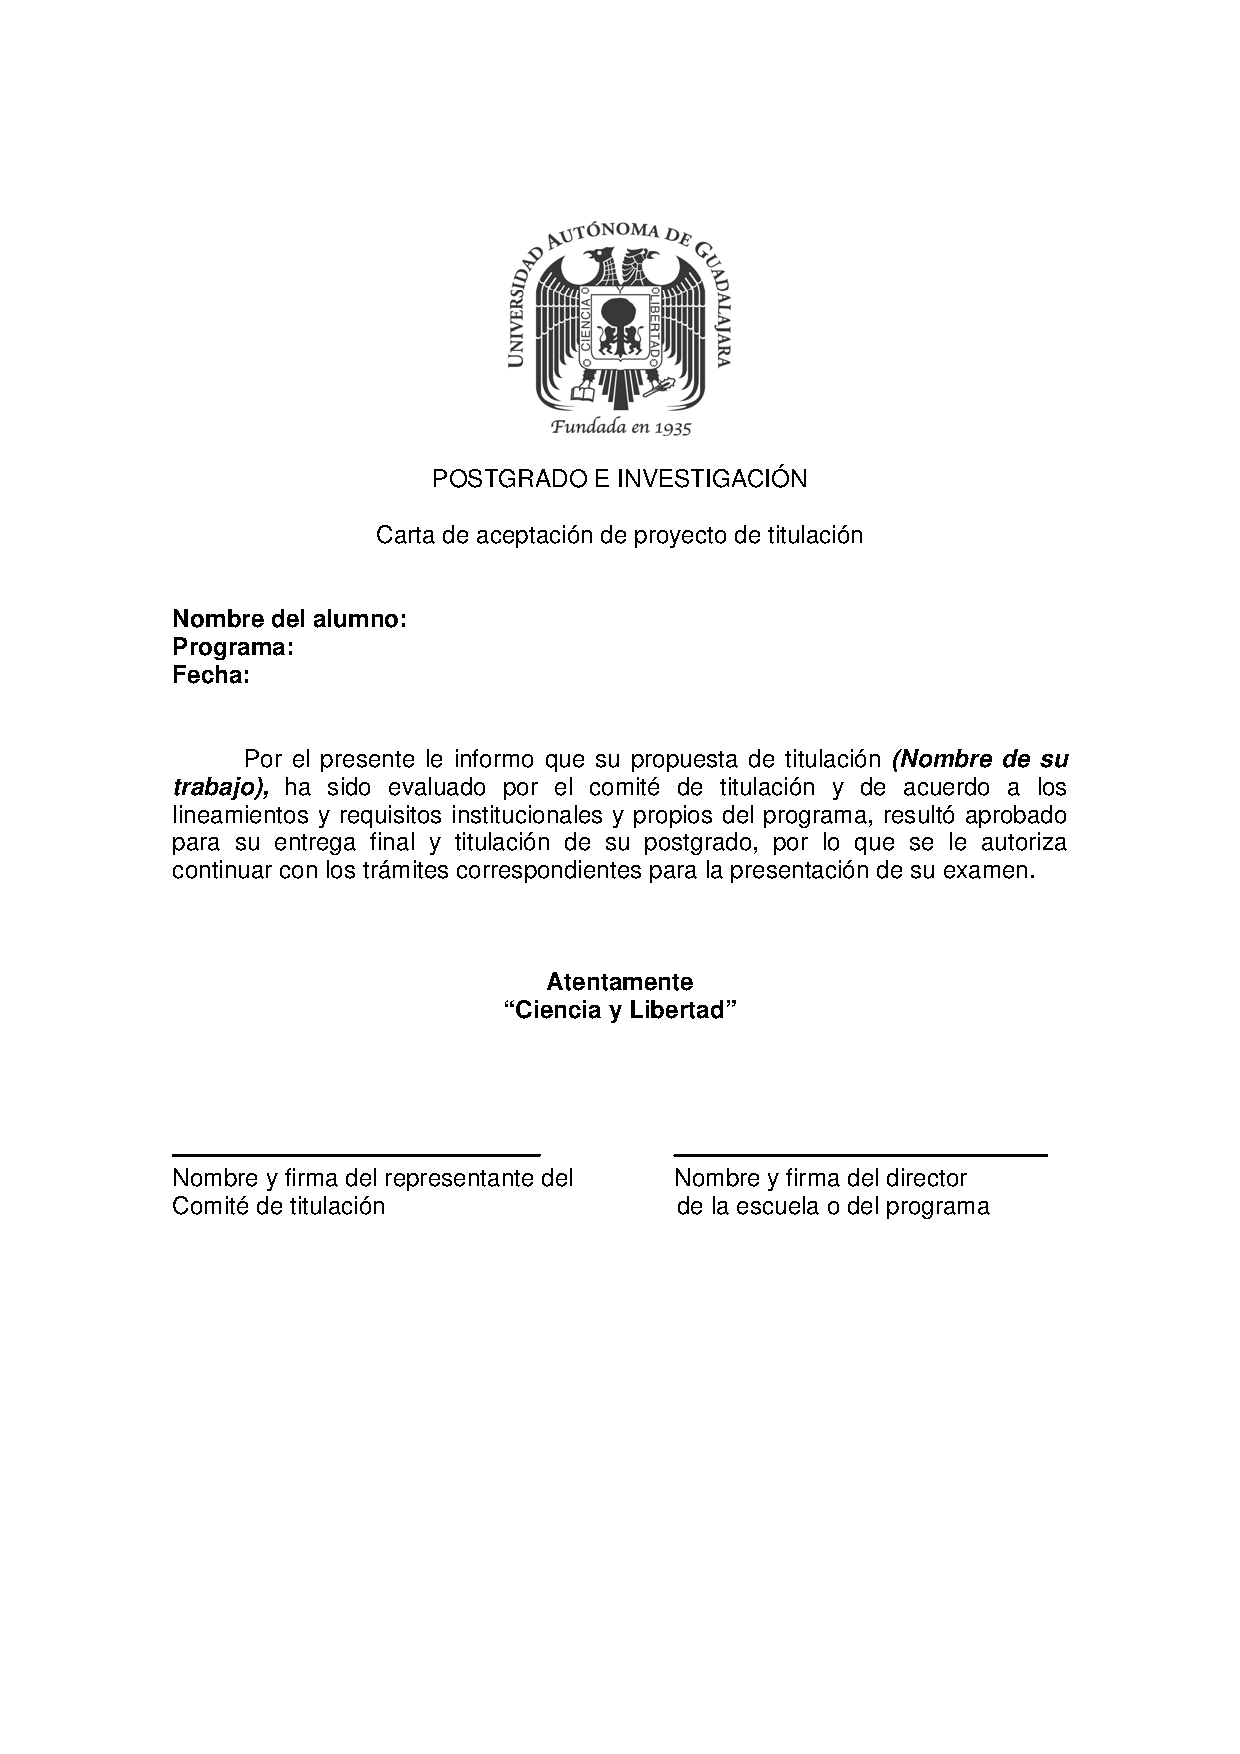
\includepdf[]{portada/cartaaceptacion.pdf} %archivo PDF y nombre de tu carta de aceptación
        
        \spacing{1.5}
        \chapter*{Abstract}
        %Abstract

El presente documento se ha elaborado con la finalidad de mostrar un ejemplo ilustrativo genérico, sin embargo se podrá elegir otros modelos de acuerdo a las características del programa académico y en concordancia con el director.
“La tesis tiene la opción de realizarse en forma interdisciplinaria, siempre y cuando se justifique de acuerdo al alcance del proyecto y en conformidad con las áreas correspondientes.” \cite{einstein}. 

        
        \chapter*{Dedicatoria}
        %Dedicatoria

Dedico este trabajo principalmente a Dios, por haberme dado la vida y permitirme el haber llegado hasta este momento tan importante de mi formación profesional. A mi madre, por ser el pilar más importante y por demostrarme siempre su cariño y apoyo incondicional sin importar nuestras diferencias de opiniones. 
        
        \chapter*{Declaración expresa}
        %Declaración expresa

La responsabilidad por los hechos, ideas y doctrinas expuestas en este proyecto corresponden exclusivamente a los directamente involucrados en su desarrollo, y el patrimonio intelectual de la misma a la Universidad Autónoma de Guadalajara.
        
        \chapter*{Agradecimientos}
        % Agradecimientos

Antes que nada agradezco a mis padres por todo el apoyo que siempre me han brindado en todo el transcurso de mis estudios y en lo largo de mi vida, sin ellos este trabajo nunca hubiera sido posible. 

También agradezco a toda mi familia por todo el apoyo que de alguna u otra forma siempre me han dado, una palabra de aliento o una frase de ánimo, gracias por estar ahí. 

        
        \tableofcontents
        
        \listoffigures
         
        \listoftables
        
        \chapter{Introducción}
        %Capítulo 1

\section{Descripción del problema} \label{descripcionproblema}

    Actualmente existe un sistema viejo donde los alumnos y profesores pueden registrar proyectos y tesis, sin embargo, este sistema al haber sido creado hace tiempo, y no seguir los estándares de calidad que hay en la actualidad ocasiona que su mantenimiento o modificación para agregar nuevas funcionalidades requiera una mayor cantidad de trabajo de codificación y pruebas, aunado a esto, la interfaz de usuario no es intuitiva ni amigable.

\section{Definición del problema} \label{definicionproblema}
    
    Dentro del proceso definido para registrar la tesis; por parte de los estudiantes, o proyectos; por parte de los profesores, existe un sistema creado hace tiempo el cual es difícil de mantener y de agregar nuevas funcionalidades ya que no sigue estándares de calidad actuales, además de tener una interfaz que no es amigable para el usuario, por esta razón se tomó la iniciativa para volver a hacer el sistema con estándares, y prácticas actuales para su codificación lo cual permitirá que se agreguen funcionalidades con mayor sencillez.

\section{Objetivo(s) de la investigación} \label{objetivoinvestigacion}
    
    \subsection{\textbf{\textit{Objetivo general}}} %Cómo hacer sub-secciones
    Elaborar el sistema de investigadores que permita a los estudiantes crear tesis, y a los profesores proyectos usando microservicios para que sea más sencillo el acoplar nuevas funcionalidades a este sistema.
    
    \subsection{\textbf{\textit{Objetivos específicos}}} %Cómo hacer sub-secciones
    \begin{enumerate}
        \item Elaborar microservicios para el crear, actualizar, eliminar y obtener información de una base de datos.
        \item Separar la funcionalidad del sistema en backend y frontend.
        \item Elaborar la base de datos relacional normalizada.
        \item Modernizar la interfaz gráfica con la cual interactúan los usuarios.
        \item Conectar los microservicios(backend) con la interfaz gráfica(frontend).
    \end{enumerate}

\section{Delimitación de la investigación} \label{delimitacioninvestigacion}

    El estudiante participará en la parte del backend para crear microservicios faltantes identificados como:
    
    \begin{enumerate}
        \item Servicio para obtener todas las tesis relacionadas a un alumno en específico.
        \item Servicio para obtener las tesis de los alumnos relacionadas a un investigador.
        \item Implementar un trabajo secundario en la base de datos que cierre las tesis al llegar a su fecha de fin para que no queden abiertas en el sistema.
        \item Servicios para manejo de perfil de usuario.
        \item Crear tablas en la base de datos para almacenar categoría de investigación, tipo de investigación, y grado.
        \item Endpoints para obtener las listas de las categorías de investigación, tipo de investigación, y grado.
        \item Elaboración de scripts para insertar datos en las tablas creadas por parte del estudiante.
    \end{enumerate}

\section{Justificación} \label{justificacion}

    La necesidad de la renovación de este sistema radica en que se agregan nuevas funcionalidades, sin embargo, después de indagar en cómo agregar dichas funcionalidades se obtuvo como respuesta que cada vez que quisieran hacer cambios, se tendría que modificar varias partes del sistema; ya que la mayoría de este es estático, por lo tanto, con la renovación se cambiará la arquitectura a una de microservicios, los cuales permiten hacer un sistema más flexible y dinámico a cambios.
    
    El trabajar con microservicios permite que se hagan módulos independientes los cuales realizan una tarea en específico, y esto da pie a integrar los módulos de manera que incluso si los requisitos van cambiando, estos no se vean afectados por los cambios requeridos.

\section{Hipótesis} \label{hipotesis}

    El nuevo sistema permite tener una flexibilidad mayor al agregar funcionalidades, o incluso modificarlas, además de que se tiene una interfaz gráfica de usuario más moderna y amigable.    % Capitulo 01
        
        \chapter{Bases Teóricas}
        %Capítulo 2

\section{Marco histórico y contextual}
    
    "La investigación en la UAG es una actividad que contribuye a dar coherencia a sus otras funciones sustantivas y tiene por objeto promover, alentar y apoyar a los esfuerzos que lleven a generar nuevo conocimiento en las áreas académicas que integran a la institución, contribuir a la solución de los problemas de la sociedad a nivel regional y nacional, mejorar la calidad del proceso enseñanza-aprendizaje para nuestros estudiantes, vinculando pertinentemente las actividades de investigación de los profesores en conformidad con la Misión, Valores y Fines de la Universidad Autónoma de Guadalajara.
    La investigación deberá ser realizada en todos los niveles educativos que ofrece la Institución y estará focalizada en proponer soluciones a los problemas planteados por los sectores productivos, social y de servicios tanto del sector público como del privado. Es por ello y siguiendo este propósito se pretende que con el Sistema de información de la Coordinación de Investigación y Desarrollo Tecnológico se tenga un registro de toda la investigación que se crean en nuestra Universidad, desde Tesis de cualquier Licenciatura o grado académico, hasta artículos, proyectos de intervención o bien cualquier tipo de investigación que sea relevante sin importar la etapa escolar en la que se esté."\cite{UAG}
    
    La página actual del sistema de investigadores de la Universidad Autónoma de Guadalajara, utiliza un diseño anticuado; antes del 2018, en el cual la mayoría de los elementos web son estáticos y, no se adaptan con fluidez a las resoluciones actuales en el año 2022, además, para incluir nuevas funcionalidades al sistema de investigadores se necesita modificar una gran cantidad de elementos web o, casi rediseñarlos, ya que la arquitectura monolítica utilizada en conjunto del patrón de diseño de Modelo-Vista-Controlador(MVC) no permite que se le agreguen nuevas funcionalidades de una manera sencilla.
    
    \begin{figure}[H]
        \centering
        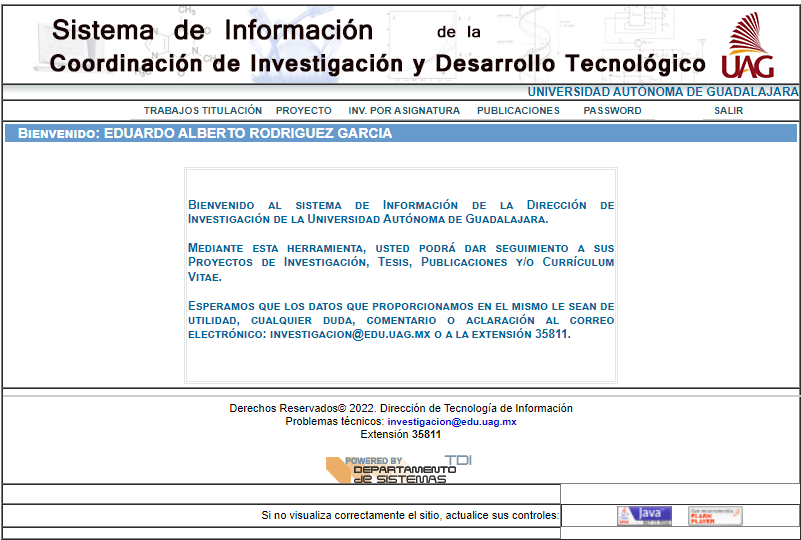
\includegraphics[width=\textwidth]{Propuesta_Plantilla_Tesis_LaTeX_UAG/imagenes/sistema_investigadores_actual.png}
        \caption{Actual sistema de investigadores.}
        \label{fig:homepage}
    \end{figure}
    
    La propuesta del equipo de trabajo liderado por la Doctora Lina María Aguilar Lobo consiste en volver a desarrollar el sistema de investigadores, pero con una nueva arquitectura y elementos que faciliten la implementación de nuevas funcionalidades. La arquitectura propuesta se compondrá de los siguientes elementos:
    
    \begin{itemize}
        \item Utilizar el patrón de diseño de Modelo-Vista-Controlador como base.
        \item Separar el desarrollo en dos partes: frontend y backend.
        \item Crear una base de datos relacional normalizada.
        \item Apoyarse de una arquitectura de micro servicios para proveer de información al frontend.
        \item Interfaz gráfica de usuario responsiva.
    \end{itemize}

\section{Marco referencial}
    \raggedbottom
    
    La arquitectura actual usada en el sistema de investigadores es de tipo monolítico, la cual se centra en un solo proveedor o servidor para interactuar con el sistema de investigadores. Esto conlleva algunas desventajas:
    
    \begin{itemize}
        \item Si alguno de los módulos del sistema de investigadores falla, esto causará que todo el sistema falle.
        \item Acoplamiento estrecho.
        \item No es sencillo escalar el sistema de investigadores; dicho en otras palabras: agregar nuevas funcionalidades.
        \item Las tecnologías usadas en el sistema de investigadores se debe de usar en todo momento. Los cambios de tecnologías son costosos en términos de tiempo y de recursos.
    \end{itemize}
    
    La mayor diferencia entre una arquitectura monolítica y una de micro servicios se puede apreciar en los diagramas siguientes:
    
    \begin{figure}[H]
        \centering
        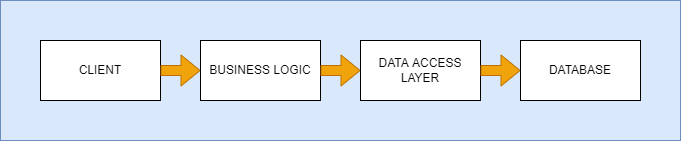
\includegraphics[width=\textwidth]{Propuesta_Plantilla_Tesis_LaTeX_UAG/imagenes/monolitico.png}
        \caption{Arquitectura monolítica.\cite{KryptonSolid}}
        \label{fig:monolitica}
    \end{figure}
    
    \begin{figure}[H]
        \centering
        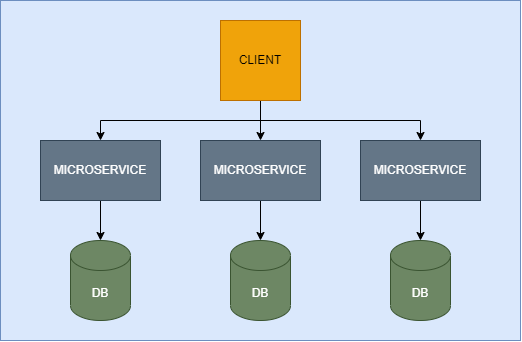
\includegraphics[width=\textwidth]{Propuesta_Plantilla_Tesis_LaTeX_UAG/imagenes/microservicios.png}
        \caption{Arquitectura basada en micro servicios.\cite{KryptonSolid}}
        \label{fig:micro-servicios}
    \end{figure}

\section{Marco Teórico}

    El nuevo sistema de investigadores que se implementa en este documento se basa en metodologías de trabajo ágiles, y así mismo de una arquitectura en el backend de micro servicios la cual traerá beneficios a la escalabilidad, acoplamiento, y gestión del sistema de investigadores.
    
    "La arquitectura de micro servicios divide los componentes del sistema en pequeños servicios autónomos que se pueden implementar y escalar de forma independiente."\cite{KryptonSolid}

    La arquitectura de micro servicios nos permite el separar cada funcionalidad en módulos específicos los cuales; al no estar estrechamente acoplados, no afectaran al sistema de investigadores si alguno presenta una falla. Además de que es más sencillo el proceso de debug y pruebas para estos módulos.

\section{Hipótesis}

    La necesidad de rehacer el sistema de investigadores yace en la habilidad de agregar nuevas funcionalidades para mejorar los procesos de los investigadores dentro de la UAG y, dado el conocimiento y habilidades de programación para backend se implementa la arquitectura de micro servicios para proveer el 100\% de la información dinámica requerida y almacenada en la base de datos a la parte del frontend la cual se encargarán otros alumnos de realizar.

\section{Definición de términos y conceptos básicos}

    \textbf{API}: Application Programming Interface \cite{jacobson2012apis}.

    \textbf{Arquitectura}: La arquitectura de software consiste en la estructura del sistema, combinado con las características arquitectónicas que el sistema debe soportar, las decisiones arquitectónicas, y finalmente los principios de diseño \cite{richards2020fundamentals}.
    
    \textbf{Arquitectura monolítica}: "El estilo arquitectónico monolítico consiste en crear una aplicación autosuficiente que contenga absolutamente toda la funcionalidad necesaria para realizar la tarea para la cual fue diseñada, sin contar con dependencias externas que complementen su funcionalidad. En este sentido, sus componentes trabajan juntos, compartiendo los mismos recursos y memoria. En pocas palabras, una aplicación monolítica es una unidad cohesiva de código." \cite{monolitic}.

    \textbf{Backend}: Hace referencia al desarrollo del lado del servidor. Se concentra en bases de datos, scripts, y arquitectura web. Contiene actividades detrás de escena que ocurren cuando se realizan acciones en el sitio web \cite{Backend}.

    \textbf{Diseño web responsivo}: El diseño web responsivo es una configuración en la que el servidor siempre envía el mismo código HTML a todos los dispositivos y se usa CSS para modificar el procesamiento de la página en el dispositivo. Los algoritmos de Google deberían detectar automáticamente esta configuración si se permite que todos los usuarios-agentes del robot de Google rastreen la página y sus elementos (imágenes, CSS y JavaScript) \cite{GoogleResponsivo}.
    
    \textbf{Frontend}: "Frontend es la parte de un programa o dispositivo a la que un usuario puede acceder directamente. Son todas las tecnologías de diseño y desarrollo web que corren en el navegador y que se encargan de la interactividad con los usuarios." \cite{Frontend}.
    
    \textbf{HTTP}: Hypertext Transfer Protocol.
    
    \textbf{Micro servicios}: La arquitectura de micro servicios es un estilo que da estructura a una aplicación como una colección de servicios con las siguientes características\cite{richards2020fundamentals}:
    
    \begin{itemize}
        \item Altamente mantenibles.
        \item Se encuentran débilmente acoplados.
        \item Desplegables independientemente; no dependen de otros servicios.
        \item Organizados por capacidades del sistema.
        \item Fáciles de probar.
        \item Pueden trabajar con diferentes tecnologías y lenguajes.
    \end{itemize}
    
    \textbf{MVC}: Modelo-Vista-Controlador.
    
    \textbf{UAG}: Universidad Autónoma de Guadalajara.
    
    \textbf{UML}: Unified Modeling Language.
    
    \textbf{URI}: Uniform Resource Identifier.    % Capitulo 02
        
        \chapter{Metodología}
        %Capítulo 3

\section{Diseño de la propuesta}

    La parte del backend del sistema de investigadores se compondrá de la siguiente figura \ref{fig:architecture}:
    
    \begin{figure}[H]
        \centering
        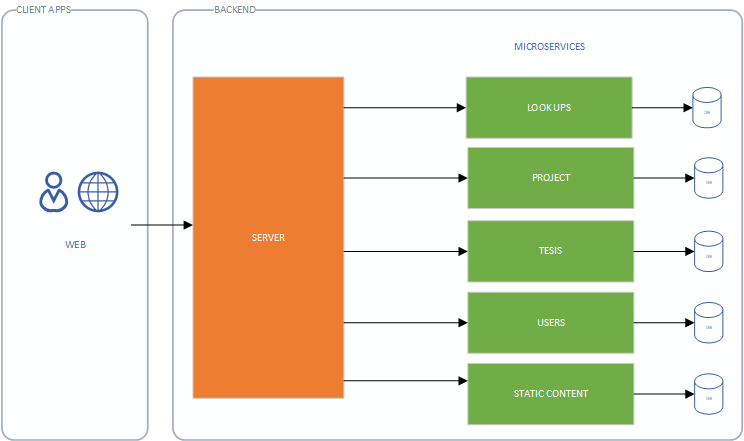
\includegraphics[width=\textwidth]{Propuesta_Plantilla_Tesis_LaTeX_UAG/imagenes/ARCHITECTURE.png}
        \caption{Arquitectura basada en micro servicios.}
        \label{fig:architecture}
    \end{figure}
    
    Con base en la figura \ref{fig:architecture} podemos apreciar que el backend va a responder a una petición hecha a través del usuario usando una interfaz gráfica, acto seguido el servidor identificará la petición para direccionarla al micro servicio correspondiente y esta hará una consulta a la base de datos para poder satisfacer la petición.
    
    Hay distintos tipos de petición que un usuario puede realizar al backend, dentro de estos se encuentran los siguientes verbos o métodos HTTP:
    
    \begin{itemize}
        \item GET: Se utiliza como lectura de datos.
        \item POST: Para poder crear nuevas entradas en la base de datos.
        \item PUT: Para la modificación de datos.
        \item DELETE: Para el borrar datos.
    \end{itemize}
    
    Los distintos tipos de usuarios que existirán son dos: Alumno e Investigador, los cuales tendrán diferentes tipos de participaciones dependiendo del trabajo al que se asignen; mostrados en la figura \ref{fig:users_table}.
    
    \begin{figure}[H]
        \centering
        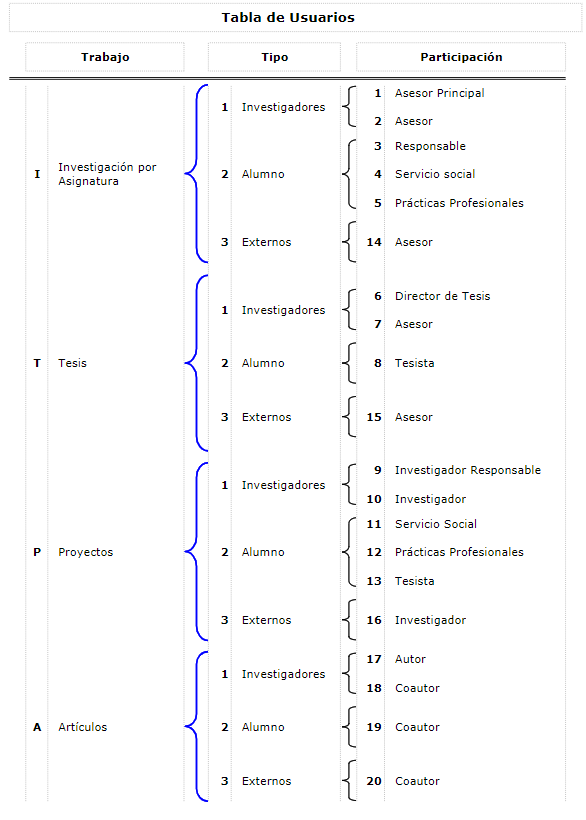
\includegraphics[width=\textwidth]{Propuesta_Plantilla_Tesis_LaTeX_UAG/imagenes/tabla_usuarios.png}
        \caption{Tabla de usuarios ordenada por trabajo y tipo de participación.}
        \label{fig:users_table}
    \end{figure}
    
    Dentro de los posibles flujos para un usuario que quiere consultar todas las tesis registradas para un alumno se puede apreciar en la figura \ref{fig:getAllTesisFromStudents} y sus pasos son los siguientes:
    
    \begin{enumerate}
        \item Realizar la petición al servidor.
        \item El servidor direccionará la petición al micro servicio o API correspondiente por medio de la URI.
        \item El micro servicio resolverá la petición del usuario y dará una respuesta con base en los datos proporcionados en la petición.
        \item El servidor obtendrá la respuesta y la regresará al usuario a través del frontend.
    \end{enumerate}
    
    \begin{figure}[H]
        \centering
        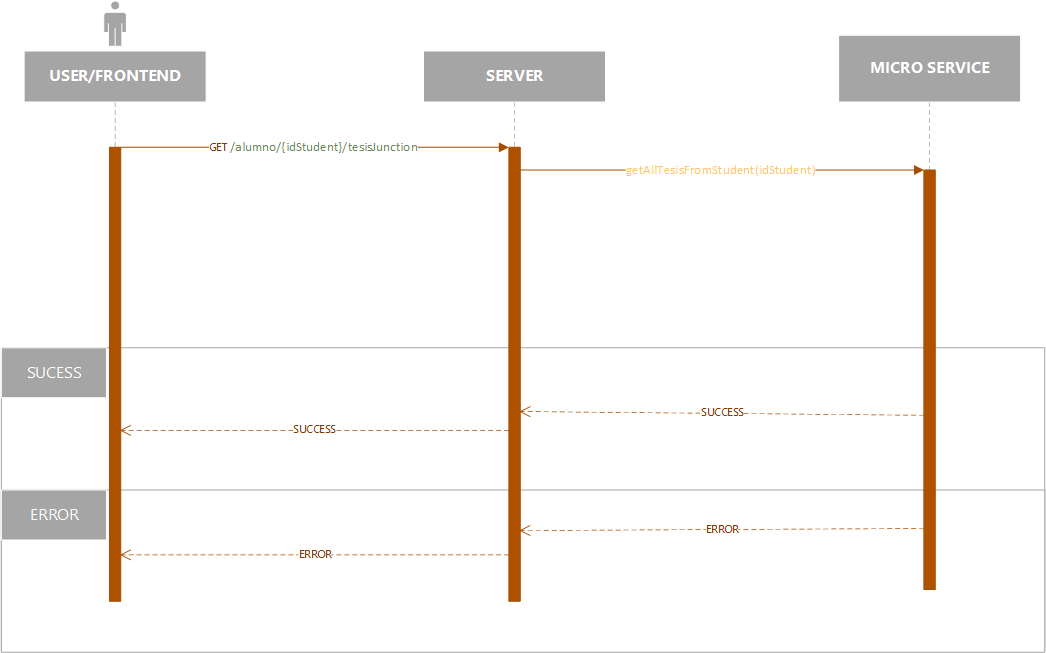
\includegraphics[width=\textwidth]{Propuesta_Plantilla_Tesis_LaTeX_UAG/imagenes/getAllTesisFromStudents_sequence_diagram.png}
        \caption{Diagrama UML para la secuencia de obtener las tesis de un alumno.}
        \label{fig:getAllTesisFromStudents}
    \end{figure}
    
    Se debe plantear un diagrama general de la propuesta del
    proyecto a realizar.
    • El objetivo es explicar en uno o varios diagramas la
    propuesta del proyecto a desarrollar, indicando el flujo de
    información, los módulos principales, la teoría relacionada,
    y los resultados esperados.
    • Debe incluir una relación lógica de los elementos que se
    consideran necesarios para dar una visión completa de la
    propuesta.
    • Debe estar orientado a los objetivos propuestos y debe
    responder a las exigencias teóricas del proyecto.

\section{Metodología}

    Se debe describir tanto la metodología como los pasos a
    seguir para el desarrollo del proyecto.
    • Se presentan los métodos o técnicas existentes a emplear
    para alcanzar los objetivos propuestos
    • Se describe cómo se hará el diseño y el desarrollo de la
    propuesta.
    • Se plantea cuál es el ambiente para realizar los
    experimentos de la propuesta.
    • Se indica cómo se evaluará el alcance de los objetivos.


\section{Cronograma}
Es la planificación y logística que se destinará a cada una
de las etapas de la investigación.
• Es el plan de actividades que muestra un orden lógico y
secuencial del proceso del proyecto.
• Deben señalarse las actividades que serán necesarias
desarrollar para cada etapa de la investigación.
• Comprende desde la presentación del protocolo hasta la
entrega del borrador de tesis.
• Se deben establecer las actividades en función del tiempo
disponible, recursos, materias que se están cursando y
políticas institucionales.

Se debe realizar un calendario tentativo de las actividades
indicadas en la metodología, indicando claramente las
tareas a desarrollar, por etapas, las cuales deberán tener un
estado actualizado (en curso, concluida).
• Se debe tener en cuenta el tiempo que se dedicará a cada
actividad. Aunque parece un detalle menor, este indicará la
factibilidad de realizar el proyecto en el tiempo determinado.
• Se deben indicar las actividades secuenciales o
dependientes y simultáneas.

Debe responder, entre otras, a las siguientes preguntas:
- ¿Cuándo se hará la recopilación de datos?
- ¿Cuándo se hará el diseño y el desarrollo (hardware o
software)
- ¿Cuándo se escribirá la tesis?
- ¿Cuándo se defenderá la tesis?

\section{Entregables}
Indicar los productos derivados del proyecto.
• Se consideran entregables los siguientes:
1. Documento Final (Tesis, Proyecto Intervención)
2. Presentación de avances en seminarios y coloquios.
3. Publicación de avances y resultados en congresos.
4. Artículos de investigación en revistas especializadas.
5. Artículos en revistas de divulgación.
6. Libros y capítulos de libros de resultados obtenidos.
7. Desarrollos y transferencias tecnológicas derivados.
8. Manuales de procedimientos.
9. Patentes, modelos de utilidad.
10. Código    % Capitulo 03
        
        \chapter{Conclusiones}
        %Capítulo 4

\section{Presentación de los resultados}

    \textbf{\textit{Descripción}}
    
    Es una argumentación fundamentada con claridad y rigor científico, donde se dan a conocer los resultados encontrados, ofreciendo respuesta a cada una de las preguntas u objetivos de la investigación \cite{knuthwebsite}.
    
    \textbf{\textit{Criterios de calidad}}
    
    Las conclusiones deben de responder a la pregunta: \textbf{¿Qué resultados se encontraron y cuáles son sus beneficios?}
    Las conclusiones deben estar redactadas con: rigor lógico, claridad y concisión de estilo, originalidad, precisión, amplitud, compatibilidad con la ética, significancia y pertinencia.
    
    Es siguiente es un ejemplo de un ecuación. Llamada Tabla \ref{tab:corr}
    
    \begin{table}[h!]
        \centering
        \begin{tabular}[c]{clccc} \hline
            \# & Corrección                 & Hird          & Nuestro                   & Factor \\  
            \hline
            1  & Frecuencia. ($Hz$)         & $1$           & $340$                     & $340$ \\
            2  & Duración ($s$)             & $1$           & $60$                      & $1/60$ \\
            3  & Área detección ($cm^2$)    & $25$          & $2.5\times 10^{-6}$       & $10^{-5}$ \\
            4  & Mancha focal ($cm^2$)      & $1$           & $1$                       & $1$ \\
            5  & Distancia ($cm$)           & $1$           & $1$                       & $1$ \\
            6  & Fuentes X-Ray              & $1$           & $1$                       & $1$ \\ \hline
        \end{tabular}
        \caption{La tabla es un ejemplo}
        \label{tab:corr}
    \end{table}

\section{Conclusiones y las recomendaciones}

    \textbf{\textit{Descripción}}
    
    Es la argumentación lógica y fundamentada, probando o desaprobando la hipótesis, y dando a conocer los beneficios o alcances de la investigación
    
    \textbf{\textit{Criterios de calidad}}
    
    Las conclusiones deben de responder a la pregunta: \textbf{¿Qué resultados se encontraron y cuáles son sus beneficios?}
    Las conclusiones deben estar redactadas con: rigor lógico, claridad y concisión de estilo, originalidad, precisión, amplitud, compatibilidad con la ética, significancia y pertinencia.    % Capitulo 04
        
        \chapter{Referencias}
        \section{Referencias documentales}

\textbf{\textit{Descripción}}

Es el listado de libros, documentos, reportes de investigación, gráficos, tablas, etc.

\textbf{\textit{Criterios de calidad}}

Debe citar técnicamente la bibliografía base de la investigación.

\section{Código fuente {\it miprograma.c}}
El siguiente código se importó directamente del archivo {\it miprograma.c}

\inputminted[breaklines=true]{c}{codigo/miprograma.c} 
        
        \bibliographystyle{ieeetr} % Formato de la IEEE
        \bibliography{bibliografia/articulos.bib,bibliografia/libros.bib,bibliografia/miscellaneous.bib}
    
    \end{document}
%-----------------------------------------------------------%